\pdfbookmark{Parallelization Approaches}{parallelization approaches}
\chapter{Parallelization Approaches}
\label{ParallelizationApproaches}

\begin{quote}
\textit{For different parallelization alternatives are presented in this chapter. For homogeneous systems, a shared memory parallelization is discussed in section \ref{Parallelization:SharedMem}, where the abstract heuristic used is shown, and the implementation and a performance analysis are presented in subsections \ref{SharedMemImplementation} and \ref{SharedMemPerformance}, respectively. For heterogeneous systems using hardware accelerators, two alternatives are presented: using GPU as an accelerator, in section \ref{Parallelization:GPU}, with its implementation and performance discussed and analyzed in subsections \ref{GPUImplementation} and \ref{GPUPerformance}; using the \intel Xeon Phi as an accelerator in section \ref{Parallelization:MIC} and its implementation discussed in subsection \ref{MICImplementation}. A software scheduler for managing workload distribution among applications for homogeneous shared memory systems is presented in section \ref{Parallelization:Scheduler}. Its implementation details and performance analysis are shown in subsections \ref{SchedulerImplementation} and \ref{SchedulerPerformance}.}
\end{quote}

As presented in chapter \ref{Application}, the critical region of the \tth application is the \ttDilepKinFit function, which execution time increases linearly with the number of variations per combination. With the initial optimizations already applied to the original application, presented in section \ref{InitialOptimizations}, the next step is to improve the performance by exploiting parallelism in the critical region. This chapter presents 4 parallelization approaches, 2 for homogeneous systems and 2 for heterogeneous systems, one using GPU and other using \intel Xeon Phi as hardware accelerators.

Although the critical region is only the \ttDilepKinFit function, the best parallelization strategy is to simultaneously perform the reconstruction of different events, as it always exploits the same degree of parallelism independent from the amount of variations performed. The event processing is data independent and no synchronizations are required, reducing the parallelization overhead. Figure \ref{fig:EventParallelization} presents a schematic representation of this parallelization approach. However, as explained in section \ref{Application:Flow}, all the event data is stored globally on the LipMiniAnalysis library, and also part on the application. Every time an event is loaded the global data is overwritten, which, in a shared memory environment, causes the intermidiate results of the event processing of one thread to be overwritten by the processing of other thread.

\begin{figure}[!htp]
	\begin{center}
		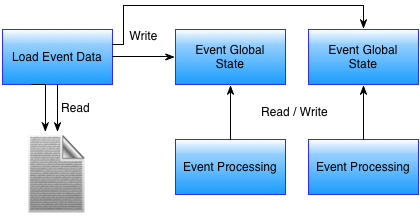
\includegraphics[scale=0.7]{../../common/img/2global_states_par.png}
		\caption{Schematic representation of the event-level parallelization model.}
		\label{fig:EventParallelization}
	\end{center}
\end{figure}

Each input file has around 1 GByte size, which allows to store all events on RAM memory. The use of a proper data structure for storing the event information would benefit the application modularity and enable the possibility of this parallelization approach. In the current implementation, each event data is loaded from the input data file before processing it. With a global data structure, the application would benefit from the performance of sequential read of the hard drives, compensating the overhead of the data structure creation. The complexity of the changes necessary to both the application source code and LipMiniAnalysis library render this approach unreliable for the timeframe of this thesis dissertation. An implementation for a classic distributed memory system, constituted by multiple CPUs on different systems, was not considered due to the thin granularity of the task to parallelize. This factor, allied to the high amount of comunications required, would induce a high overhead that would greatly limit the performance improvements. If the application handled a private memory state for each event, the parallelization proposed above would be reliable to implement on this kind of environments.

The \ttDilepKinFit handles mostly private data to the function. The global data modified by this function can be controlled without any modifications to the LipMiniAnalysis library. Looking at the information presented in section \ref{ComputationalCharactrization}, specifically in figure \ref{fig:KinFitGraph}, most performance gains are expected to occur for 16 to 512 variations per combination as for that problem size the \ttDilepKinFit occupies most of the application execution time.

The \ttDilepKinFit execution is irregular, meaning that, depending on the event to be reconstructed, its execution time may vary. This is caused by the number of Bottom Quark jets and leptons combinations, which differs between events. Also, the execution flow is dependent on the kinematical reconstruction. If the \ttbar system has a possible reconstruction, \ttDilepKinFit attempts to reconstruct the Higgs Boson. If not, the Higgs Boson is not reconstructed reducing the function execution time. This translates in an irregular workload likely to affect the performance if the load balancing strategy is not suited for the problem.

The kinematical reconstruction is performed on the \dilep function. The \ttbar system obeys a set of properties expected from the Top Quark theoretical model. To reconstruct both Top Quarks it is required to know the characteristics of all resultant particles from their decay. However, since the neutrinos do not react with the detector, and their characteristics are not recorded and it is necessary to infer them using various properties of the system, such as momentum and energy conservation. Once the neutrinos characteristics are determined, the Top Quarks are possible to reconstruct. \dilep analitically solves a system of 6 equations to infer the neutrinos characteristics and then reconstruct the Top Quarks. The function is dependent on only one class from ROOT, \texttt{TLorentzVector}, and only handles data private to the function.

\section{Shared Memory Parallelization}
\label{Parallelization:SharedMem}

The left scheme of figure \ref{fig:SeqPipeline} illustrates the current workflow of the \ttDilepKinFit. The best approach is to parallelize the loop that iterates through all the jets/leptons combinations. However, the computation of the combinations cannot be performed in parallel as for chosing one combination it is necessary to know all the combinations chosen so far. Also, the combinations information is stored globally to the application so a data structure must be created to allow reconstructions of different combinations to be performed simultaneously.

\begin{figure}[!htp]
	\begin{center}
		\raisebox{-0.5\height}{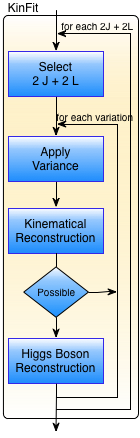
\includegraphics[scale=0.7]{../../common/img/sequential_kinfit.png}}
		\raisebox{-0.5\height}{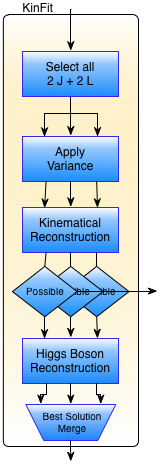
\includegraphics[scale=0.7]{../../common/img/parallel_kinfit.png}}
		\caption{Schematic representation of the \ttDilepKinFit sequential (left) and parallel (right) workflows.}
		\label{fig:SeqPipeline}
	\end{center}
\end{figure}

For the shared memory parallelizaiton, the number of parallel tasks will be equal to the number of total reconstructions to process, which is the number of combinations times the number of variations per combination. This small granularity of the tasks allows for the scheduler to better distrubute the work among the threads. Each task has a combination assigned and it applies a variation and reconstructs it. The result of the reconstruction is stored in a memory state private to the task so that, after all variations of all combinations are computed, a reduction is performed to find the best solution among all tasks. The reduction can also be parallelized, reducing its complexity from \textit{O(N)} to \textit{O($log_{2}$(N))}, where \textit{N} is the number of elements to reduce.

\begin{figure}[!htp]
	\begin{center}
		\raisebox{-0.5\height}{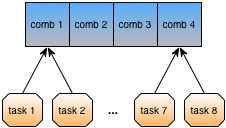
\includegraphics[scale=0.7]{../../common/img/parallel_methodology.png}}
		\raisebox{-0.5\height}{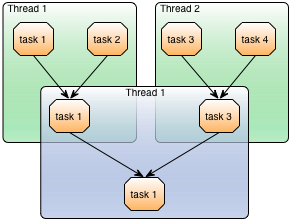
\includegraphics[scale=0.7]{../../common/img/parallel_reduction.png}}
		\caption{Schematic representation of the parallel tasks accessing the shared data structure (left) and the new parallel reduction (right).}
		\label{fig:ParallelMethodology}
	\end{center}
\end{figure}

Figure \ref{fig:ParallelMethodology} presents the parallelization strategy using concurrent tasks sharing the combinations data structure and the strategy for the parallel reduction. This modifications to the workflow are schematized in the right scheme of figure \ref{fig:SeqPipeline}. As stated before, chosing the combinations and building the data structure cannot be performed in parallel. This reduces the size of the parallel region and adds an extra overhead to each \ttDilepKinFit call. This overhead is also increased by the best solution merge, which does not occur in the sequential application.

\subsection{Implementation}
\label{SharedMemImplementation}

The implementation process was iterative, where every major change is tested in terms of performance and correctness of the application output before proceeding to the next change. Since the application code is very complex has a heavy global state, small modifications, specially when introducing parallelism, can completly alter the application behavior and affect the results. The OpenMP library was used to implement the parallelization as it is the most adopted among scientists and easier to include in C/C++-like applications such as \tth. It offers many of the functionalities required by this parallelization strategy, such as parallel reductions, various workload schedulers and explicit thread management and synchronization primitives. Also, OpenMP allows for the number of threads to be defined by environment variables, without any changes to the code, which eases the user interaction without changing its input parameters.

Each step of the \ttDilepKinFit workflow (see figure \ref{fig:SeqPipeline}, left image) was individually parallelized to control the impact of the concurrent tasks on the overall behavior. Then, all the parallel regions were concatenated, resulting in the workflow presented in figure \ref{fig:SeqPipeline}, right image. At this point the main concern was the correcteness of the application, rather than its performance.

The first task performed by \ttDilepKinFit is selecting all possible combination. This sequential task can be performed simultaneously to building the data structure holding its information. The total amount of combinations, which depends on the amount of jets and leptons $n$, pairing two jets with two leptons, being $k = 4$, in the same combination regardless of their order, i.e. $(j_1, j_2) = (j_2, j_1)$, is, according to the formula for mathematical combinations, presented in equation \ref{eq:Combination}. The average number of combinations for the input data file is 131.

\begin{center}
	\begin{equation}
		\binom{n}{k} = \frac{n!}{k!(n - k)!} \mbox{, with k = 4 then } \binom{n}{4} = \frac{n!}{8(n - 4)!}
		\label{eq:Combination}
	\end{equation}
\end{center}

All the information of the Bottom Quark jets and leptons (ROOT \texttt{TLorentzVector} class instances), as well as other control and auxiliary information is stored in a class built for this purpose. The function responsible for the variation of the parameters was implemented as a method of this class, increasing the modularity of the code. Each task creates a local copy of the combination to apply the variation and reconstruct. This keeps the integrity of the original combination parameters, allowing it to be varied any number of times. Otherwise, applying a variation to an already varied combination would result in inaccurate physics results.

The size of one data structure element is 2 kB, making an average data structure size of 262 kB per event. Even though the data structure size is not big, the overhead of its construction might prove to be a factor limiting the performance. Note that the number of variations to perform does not affect the size of the data structure.

One of the major problems of this parallelization is to control the accesses to the global state on the LipMiniAnalysis library. In \ttDilepKinFit, 34 global variables of mostly ROOT classes instances and vectors, are read and writen inside the parallel region. The access to this variables can be serialized but that would alter the behavior of concurrent tasks reconstructing different variations of the same combination. Further analysis of the source code reveals that even though these variables are global they are only modified by the \ttDilepKinFit function and their purpose is only to store intermidiate results. The most efficient solution is to create a local copy of the global state in each thread (note that a thread contains one or more parallel tasks), removing any data dependencies and avoiding serial accesses that can cause contention on the shared resources and degrade the performance.

After reconstructing all variations of all combinations for an event only the best reconstruction is necessary. Each solution quality is measured by a scalar value, computed comparing the reconstructions to the theoretical model, and the higher the value the better the reconstruction. The best solution is a set of 16 \texttt{TLorentzVectorWFlags} class instances (from LipMiniAnalysis), an extension to the ROOT \texttt{TLorentzVector} class, and a scalar with the solution quality. A class was created holding all this information and implementing all comparator operations, which increases the implementation overhead but reduces the complexity of the reduction process. Since OpenMP only supports parallel reduction for scalar values, a custom parallel reduction was implemented. The reduction is not performed among all tasks but rather among the threads used; during the reconstructions, each thread automatically holds the information of only the best solution, which is then used in the reduction, diminishing the amount of elements to compare. After the reduction, the best solution information is copied to the global state.

The algorithm used for the reduction is simple. The threads are grouped two by two in each level of the reduction tree and their solutions are compared. The thread with the lower id keeps the best solution of its pair. Threads which do not have a pair check a queue of unpaired threads and pick one. If the queue is empty, they are put in there. An example reduction is presented in figure \ref{fig:Reduction}.

\begin{figure}[!htp]
	\begin{center}
		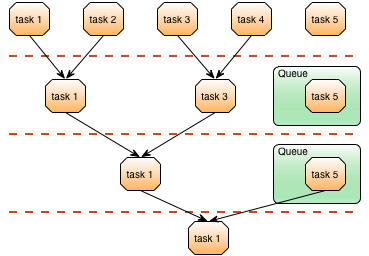
\includegraphics[scale=0.7]{../../common/img/parallel_reduction_example.png}
		\caption{Schematic representation of a possible best solution reduction in \ttDilepKinFit.}
		\label{fig:Reduction}
	\end{center}
\end{figure}

As mentioned in section \ref{InitialOptimizations}, the pseudo-random number generator used for applying the variations is the \texttt{TRandom3} ROOT class. It uses the Mersenne Twister algorithm which heavily depends on a huge global state. Concurrent threads cannot use the same global state because one thread random number generation would influence the other thread generation, requiring serialization of the process. However, it is perfectly possible that different threads use different global states, eliminating the resource contention and correlations between random numbers. In this implementation, each thread has its own instance of the \texttt{Trandom3} class, ensuring that there are no global states shared and allowing for thread safe pseudo-random number generation.

OpenMP offers a set of different schedulers, from which the most relevant are the static and dynamic schedulers. The static scheduler defines the number of parallel tasks that each thread will process prior to the parallel region execution. This scheduler has a small processing footprint and is very efficient for balancing regular workloads. For irregular workloads, such as \ttDilepKinFit, the static scheduler porduces a poor workload balance, which may affect the performance. The dynamic scheduler requires more computational power but performs a better job at balancing irregular workloads. The scheduler monitors the execution load of each thread and maps the tasks to the threads at runtime. Parallel implementations performance using both schedulers are analyzed and compared in subsection \ref{SharedMemPerformance}.

\intel VTune tool was used to analyze and identify the bottlenecks of the parallel implementation. With the help of this profiler, the constructor of the data structure of the combinations was identified as the main performance bottleneck. When analyzing the data structure source code, its evident that some of its parameters are only read and not modified during each event processing. Instead of copying these parameters for each element of the data structure, it is possible to use a pointer to their memory position in the global state. The access to this data can be parallel as it is read-only. However, it may decrease the performance when using various CPUs, as threads in one CPU may have to access data in other CPU, causing NUMA accesses. The performance of this implementation, addressed as pointer version, is compared against the previous implementation, addressed as non-pointer version, in subsection \ref{SharedMemPerformance}.

\subsection{Performance analysis}
\label{SharedMemPerformance}

The performance analysis of the various shared memory implementations will be presented in this section. Many metrics for evaluating performance will be used, such as speedup and throughput, always compared to the original application, and the results will be analyzed and discussed. The compute-711 system was used to conduct the tests in this section.

Figures \ref{fig:RegularSpeedup} and \ref{fig:PointerSpeedup} present the speedups for various number of threads, using one and two CPUs, with and without Multithreading\footnote{Refer to appendices \ref{App:TestEnv} and \ref{App:TestMethodology} for test system and methodology characterization.}. The maximum theoretical speedup is also presented in figure \ref{fig:AmdahlSpeedup}, for comparing the efficiency of the parallelization with the already optimized original sequential application. It is expected that the overhead of creating the data structure and merging the results may slightly affect the performance, specially for a small number of variations.

\begin{figure}[!htp]
	\begin{center}
		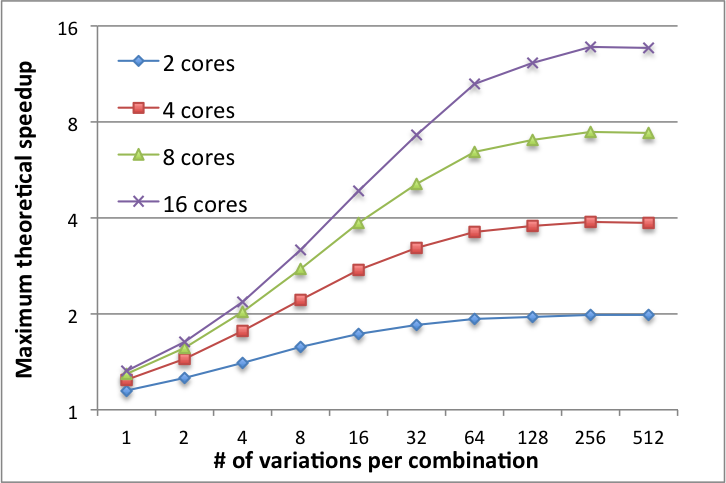
\includegraphics[scale=0.7]{../../common/graphs/amdahl_speedup.png}
		\caption{Theoretical speedup (Amdahl's Law) for various number of cores.}
		\label{fig:AmdahlSpeedup}
	\end{center}
\end{figure}

The maximum theoretical speedup calculation, presented in figure \ref{fig:AmdahlSpeedup}, is based on the Amdahl's Law \cite{AMDAHL} which states the maximum attainable speedup depends on the number of processors and the percentage of the execution time spent on the region to parallelize. The efficiency of the parallelization of an application can be measured by the difference of the speedup curve to the respective Amdahl's speedup curve. The Amdahl's Law was calculated for the original application with the initial optimizations to assess the efficiency of only the parallelization implementation.

\begin{figure}[!htp]
	\begin{center}
		\raisebox{-0.5\height}{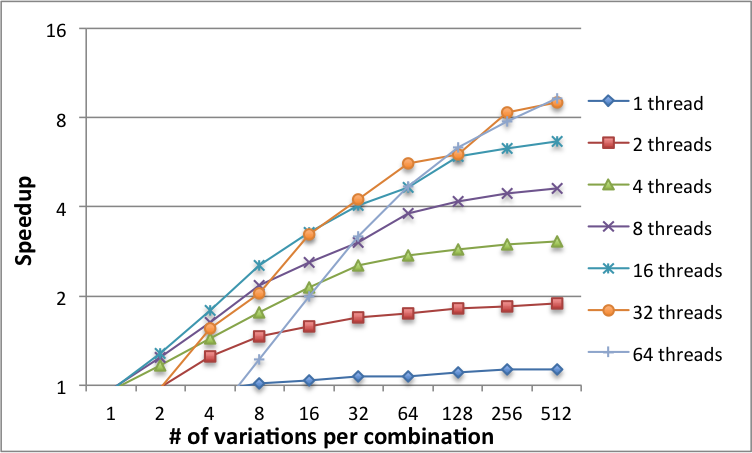
\includegraphics[scale=0.6]{../../common/graphs/speedup_nonpointer_static.png}}
		\raisebox{-0.5\height}{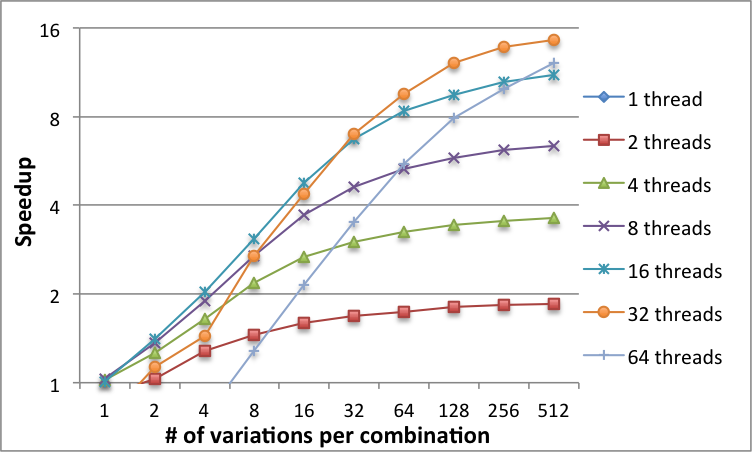
\includegraphics[scale=0.6]{../../common/graphs/speedup_nonpointer.png}}
		\caption{Speedup for the parallel non-pointer version of \tth application with static (left) and dynamic (right) scheduling.}
		\label{fig:RegularSpeedup}
	\end{center}
\end{figure}

Even with the performance increase provided by the optimizations in section \ref{InitialOptimizations}, for a low number of variations per combination the overhead of the thread management, data structure creation and best solution merge is too high and causes the application to be slower than the original. With the increase of threads, the thread management overhead increases and the performance is even lower. Overall, the best results are obtained using the dynamic scheduler. The dynamic scheduler overhead is evident when looking for the results using 1 thread, where the overhead difference is only due to the schedulers: for 8 and more variations the static scheduler implementation offers speedups, while the dynamic scheduler implementation performance is always worse than the original application. Using all available cores (16 threads) the speedup is 6.7 and 9.2, for the static and dynamic scheduler versions respectively, for the best case of 512 variations. The use of hardware multithread (32 threads) benefits the performance in both cases, but the speedup is bigger for the dynamic scheduler implementation. It allows hiding the high latency of RAM memory acesses by scheduling threads which are ready to execute while others are idle waiting for the data. Multithreading managed by software (64 threads) offers speedups better than using 16 threads, but only high number of variations, such as 256 and 512. The best efficiency (speedups closest to the theoretical maximum) is obtained for 2, 4 and 32 threads of the dynamic scheduler implementation.

\begin{figure}[!htp]
	\begin{center}
		\raisebox{-0.5\height}{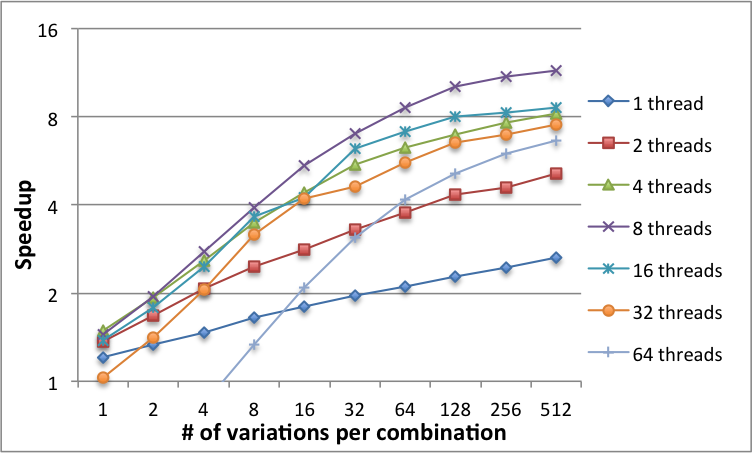
\includegraphics[scale=0.6]{../../common/graphs/speedup_pointer_static.png}}
		\raisebox{-0.5\height}{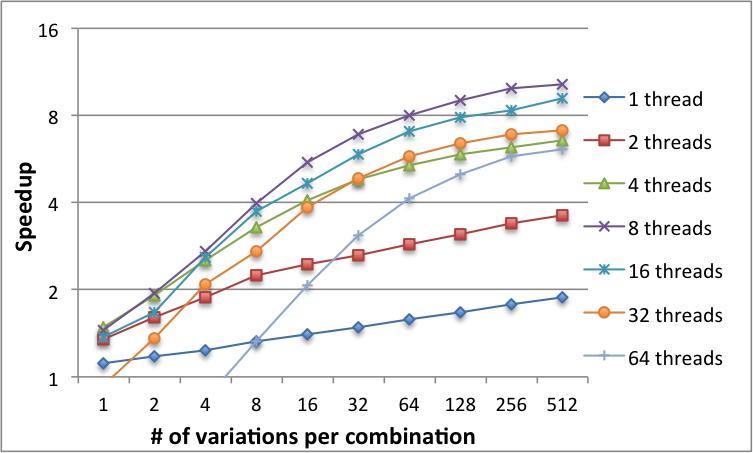
\includegraphics[scale=0.6]{../../common/graphs/speedup_pointer.png}}
		\caption{Speedup for the parallel pointer version of \tth application with static (left) and dynamic (right) scheduling.}
		\label{fig:PointerSpeedup}
	\end{center}
\end{figure}

Similar to the non-pointer version, the dynamic scheduling provides the best performance for high number of threads in the pointer version. However, for 2, 4 and 8 threads the low overhead of the static scheduler gives this implementation an advantage against the dynamic scheduler version. When both CPUs are used, the performance of the static scheduler version degrades relatively to the dynamic scheduler. The difference between the overheads of the two schedulers is evident when comparing both implementations using only one thread. The most important results refer to the efficiency of the static scheduler implementation for 2, 4 and 8 threads, as they present superscalar speedup\footnote{Superscalar speedup occurs when the speedup is higher than the number of CPU cores used.}, mostly due to the pseudo-random number generation optimizations allied to the low overhead of constructing the data structure, opposed to the higher overhead of the non-pointer version. It was not possible to test the speedup of only one CPU using multithreading as the current implementation of OpenMP does not allow to manually match the threads to the cores, and multithreading is only enabled when all available physical cores are occupied.

\begin{figure}[!htp]
	\begin{center}
		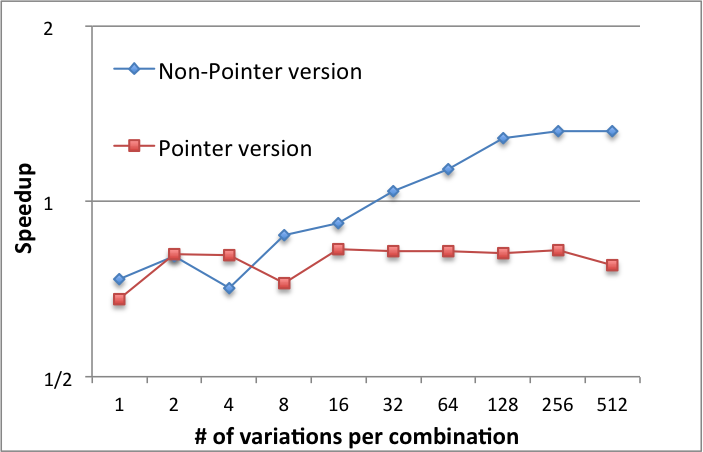
\includegraphics[scale=0.7]{../../common/graphs/ht_speedup.png}
		\caption{Speedup provided by using hardware multithreading for the non-pointer version.}
		\label{fig:HTSpeedup}
	\end{center}
\end{figure}

The speedup provided by the use of hardware multithreading, presented inf figure \ref{fig:HTSpeedup}, which helps to improve the CPU resource usage by scheduling multiple threads per core, is only noticeable for 32 or more variations in the non-pointer implementation. It provides a speedup up to 1.3 over using only 1 thread per core, by diminishing the impact of high latency RAM memory accesses. In the pointer implementation, hardware multithreading degrades performance due to the usage of pointers to shared memory, resulting in the increase of the latency of memory accesses proportional to the number of threads usedwhen using multiple CPUs.

Considering both dynamic scheduler non-pointer and static scheduler pointer implementations, which are the best performing, the non-pointer version offers the best speedup for 32 threads. However, the best efficiency is obtained by the pointer version for 2, 4 and 8 threads, due to the reduced overhead of constructing the data structure. It provides a speedup of 11.5 for 8 threads and 512 variations, only matched by the non-pointer implementation using 16, 32 and 64 threads. For higher number of threads the performance does not increase, which is an expected behavior since threads in different CPUs share a pointer to the same data. The non-unified memory accesses to shared memory degrade the performance as the data cannot be properly stored in the cache preventing a set of memory management optimizations. Chosing the best implementation depends on the system, since the non-pointer version is best for multi-CPU systems while the pointer version is best for single CPU systems. VTune did not identify more bottlenecks on the application code, not considering functions on the LipMiniAnalyisis library.

\begin{figure}[!htp]
	\begin{center}
		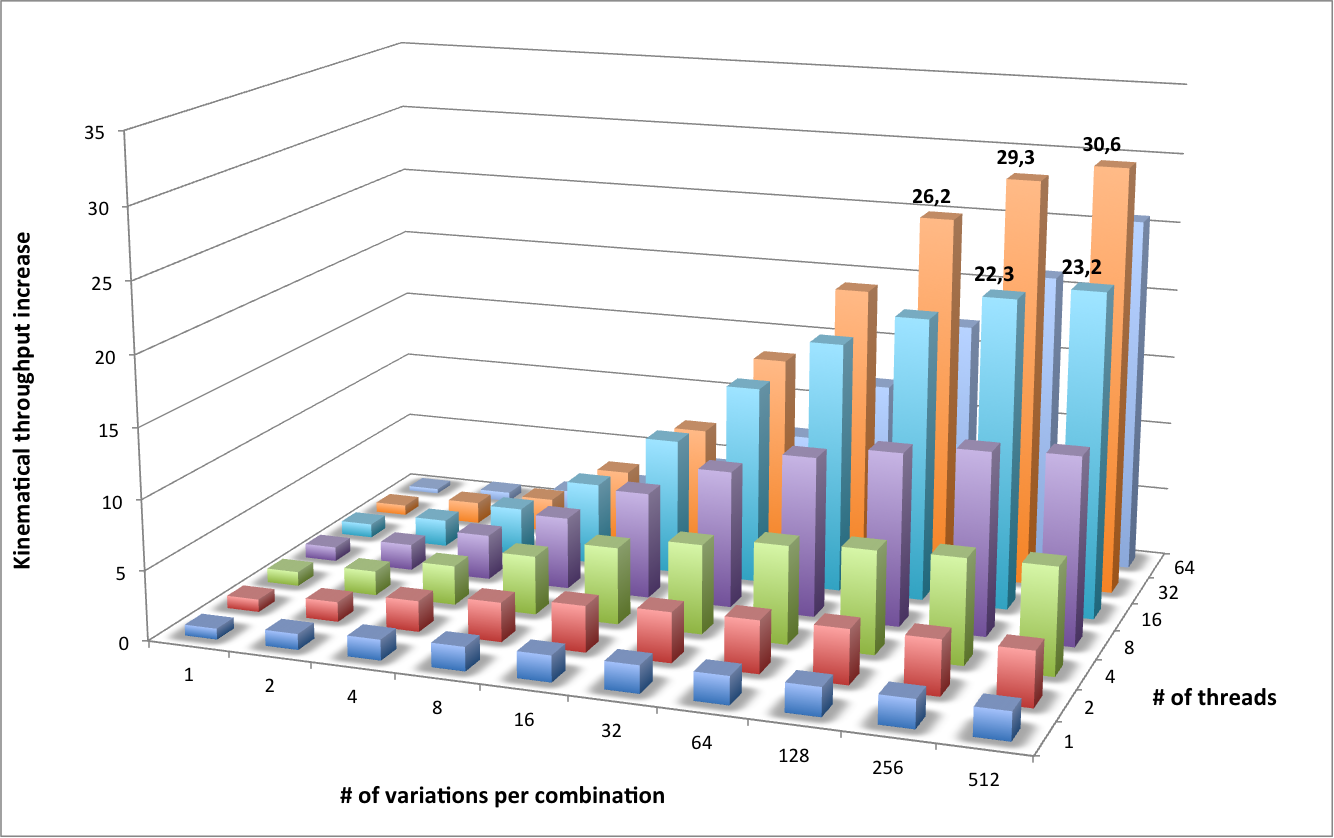
\includegraphics[scale=0.6]{../../common/graphs/dilep_throughput.png}
		\caption{Kinematical reconstruction throughput for various number of variations and threads.}
		\label{fig:DilepThroughput}
	\end{center}
\end{figure}

One possible metric to measure the increase of processing throughput in the \ttDilepKinFit is the increase of kinematical reconstructions performed relatively to the sequential application. Only the kinematical reconstruction is suitable for this purpose as it is always executed, opposed to the Higgs Boson reconstruction which is only performed if the \ttbar system is reconstructed. The speedup of the kinematical reconstruction relatively to the original application is presented in figure \ref{fig:DilepThroughput}. The non-pointer implementation performs up to 30 times more kinematical reconstructions than the original application in the same time, for 512 variations and 32 threads. This value does not translate directly into overall application speedup at this only considers a regular task inside the bigger and irregular \ttDilepKinFit.

\begin{figure}[!htp]
	\begin{center}
		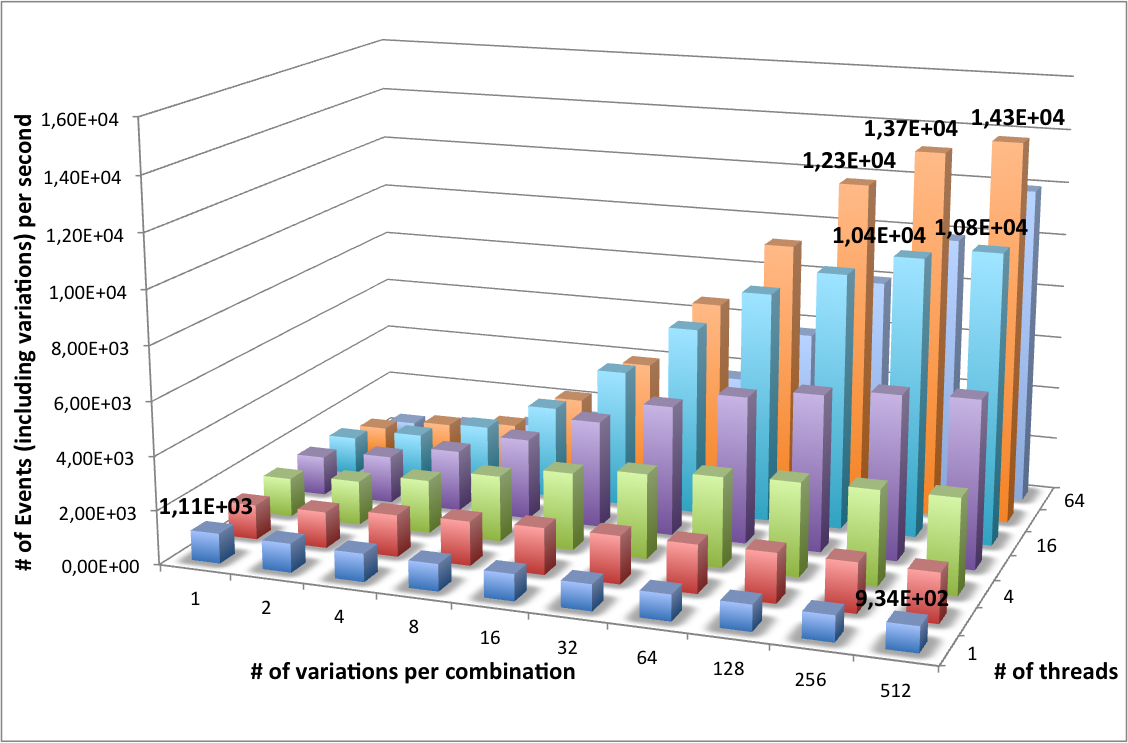
\includegraphics[scale=0.6]{../../common/graphs/throughput.png}
		\caption{Event processing throughput for various number of variations and threads of the non-pointer version.}
		\label{fig:EventThroughput}
	\end{center}
\end{figure}

\begin{figure}[!htp]
	\begin{center}
		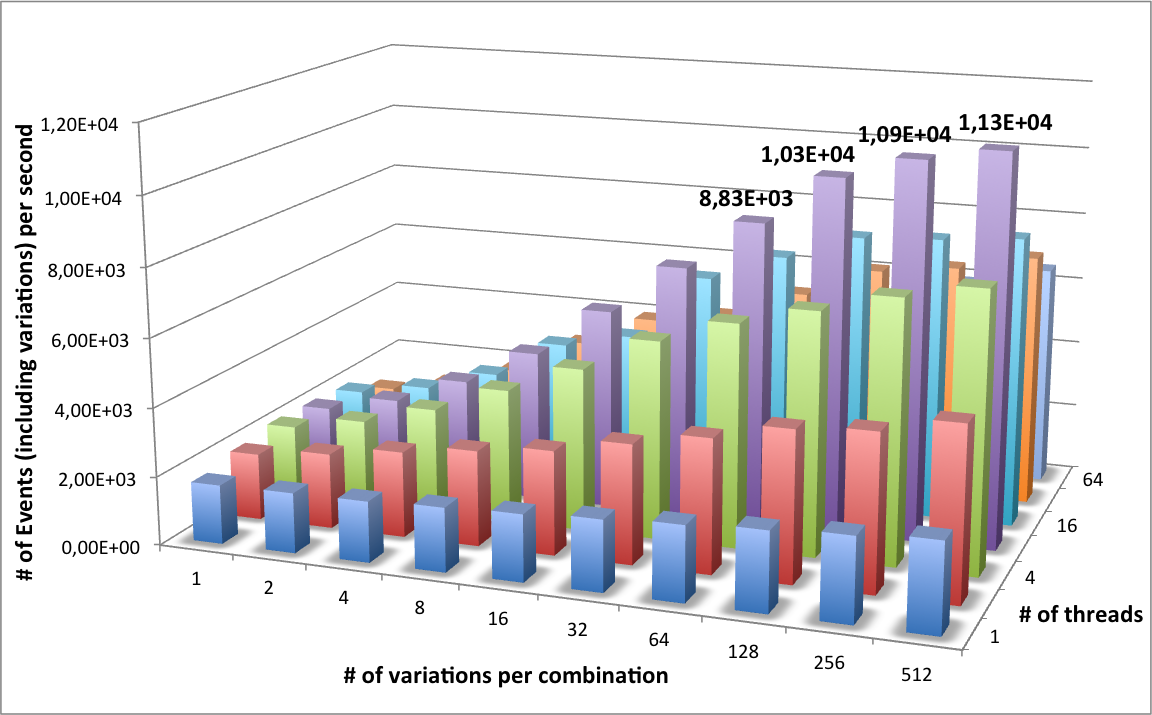
\includegraphics[scale=0.6]{../../common/graphs/throughput_pointer.png}
		\caption{Event processing throughput for various number of variations and threads of the pointer version.}
		\label{fig:EventThroughputPointer}
	\end{center}
\end{figure}

One of the concerns for research groups is the amount of events that their applications are able to process. Figures \ref{fig:EventThroughput} and \ref{fig:EventThroughputPointer} present the event throughput for the non_pointer and pointer versions, respectively. The event processing throughput is considered to be all events in the input data file, as well as each individual variation reconstructions of those who reach cut number 20 of \tth. The sequential, already optimized, application is presented in the \"1 thread\" line in both graphs. For 512 variations and 32 threads the event throughput is 14300 events per second for the non-pointer version, which is 15 times higher than the original for the same number of variations. However, the pointer version always has a higher throughput, more evident for 4 and 8 threads.

\subsubsection{Performance analysis on various computational systems}
\label{SharedMemPerformanceVarious}

Scientific computer clusters are not always made of high end computing nodes, such as the compute-711 test system used in this chapter. A simpler performance analysis on 3 dual-socket test systems common among research groups is presented in this subsection. Only the speedup and execution time will be compared, as an in-depth analysis was already made in section \ref{SharedMemPerformance}.

Only the two best implementations, non-pointer with static scheduling and pointer with dynamic scheduling, are tested for three different number of threads: one per core using one CPU; one per core using both CPUs; one per hardware thread if hardware multithreading is supported. The test systems used are the compute-401, compute-511 and compute-601 nodes of the SeARCH cluster\footnote{See appendix \ref{App:TestEnv} for the characterization of all test systems.}.

\begin{figure}[!htp]
	\begin{center}
		\raisebox{-0.5\height}{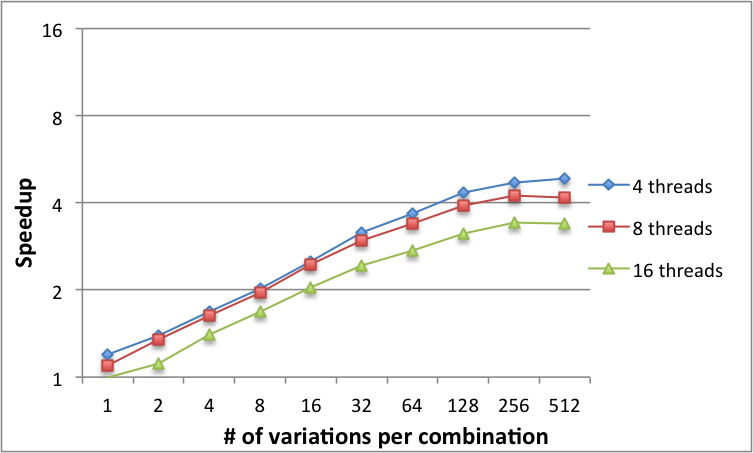
\includegraphics[scale=0.6]{../../common/graphs/speedup_pointer_401.png}}
		\raisebox{-0.5\height}{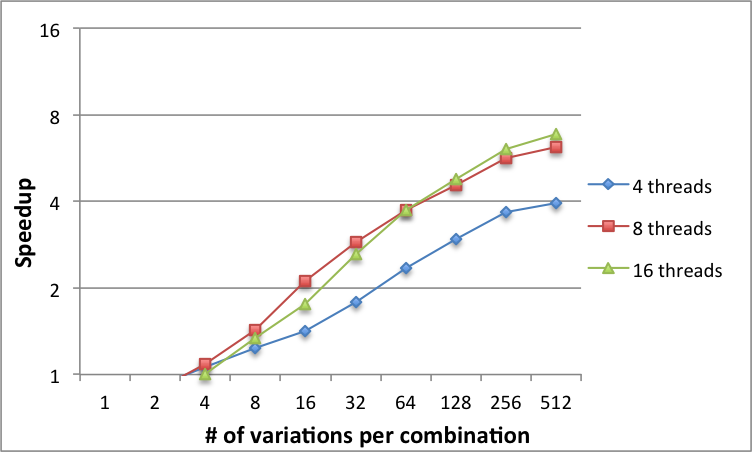
\includegraphics[scale=0.6]{../../common/graphs/speedup_nonpointer_401.png}}
		\caption{Speedup of the \tth application for pointer static (left) and non-pointer dynamic (right) scheduler implementations in the compute-401 node.}
		\label{fig:Speedup401}
	\end{center}
\end{figure}

Much like the compute-711, the best performance is obtained on the non-pointer version for 16 threads (using all multithreaded cores). However, the multithreading gains are not as significative as with the the compute-711 system. The best efficiency is obtained using 4 threads, the entire cores of one CPU, for the pointer version, attaining a speedup of 4.8 for 512 threads.

\begin{figure}[!htp]
	\begin{center}
		\raisebox{-0.5\height}{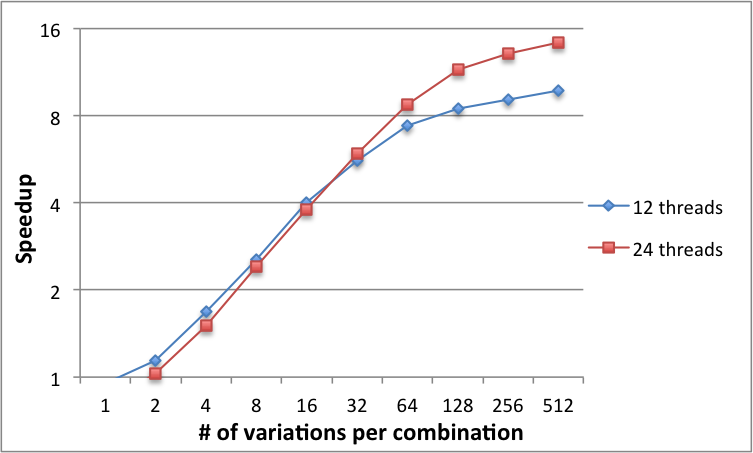
\includegraphics[scale=0.6]{../../common/graphs/speedup_pointer_511.png}}
		\raisebox{-0.5\height}{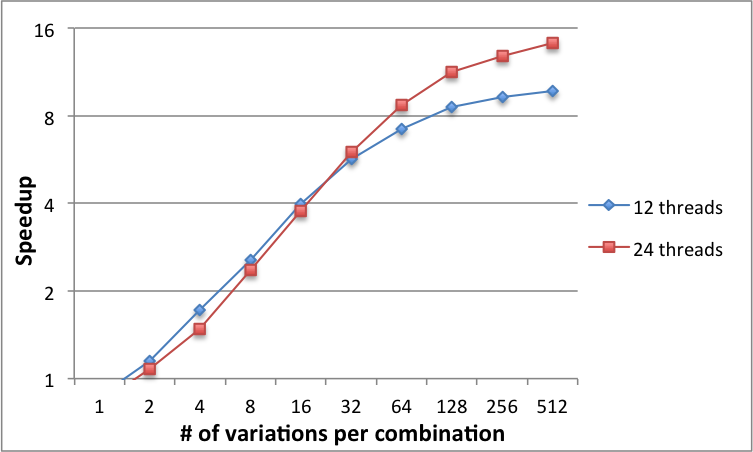
\includegraphics[scale=0.6]{../../common/graphs/speedup_nonpointer_511.png}}
		\caption{Speedup of the \tth application for pointer static (left) and non-pointer dynamic (right) scheduler implementations in the compute-511 node.}
		\label{fig:Speedup511}
	\end{center}
\end{figure}

The speedups for the compute-511, in figure \ref{fig:Speedup511}, are very similar in the two versions, with a slight advantage for the pointer version. However, for 24 threads it is far from the peak performance as the system as a total of 24 physical cores. This is due to the poor memory management characteristic of AMD CPUs, which is specially evident in a NUMA accesses. Even though the speedup is quite good for 12 threads, the execution time is the worse of all the systems, as presented in figure \ref{fig:ExecTimes}.

\begin{figure}[!htp]
	\begin{center}
		\raisebox{-0.5\height}{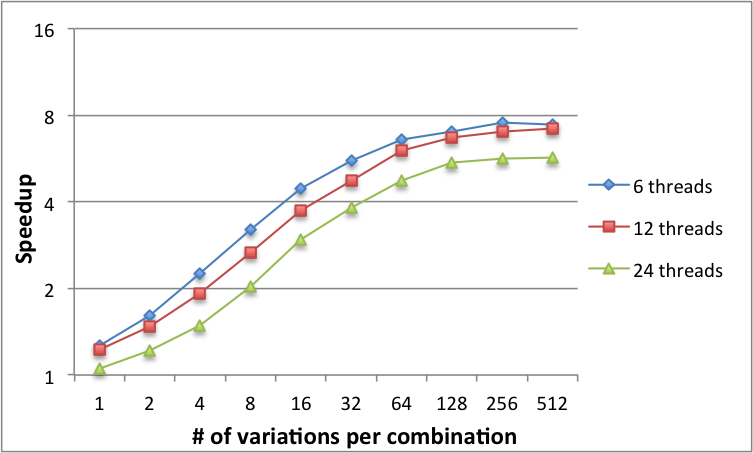
\includegraphics[scale=0.6]{../../common/graphs/speedup_pointer_601.png}}
		\raisebox{-0.5\height}{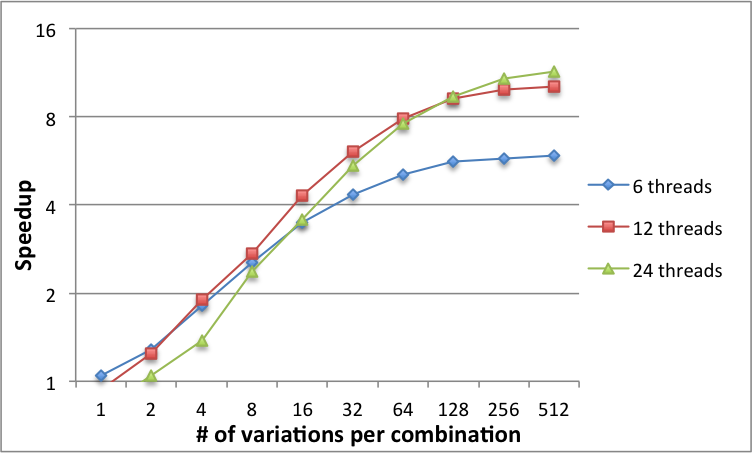
\includegraphics[scale=0.6]{../../common/graphs/speedup_nonpointer_601.png}}
		\caption{Speedup of the \tth application for pointer static (left) and non-pointer dynamic (right) scheduler implementations in the compute-601.}
		\label{fig:Speedup601}
	\end{center}
\end{figure}

The compute-601 system behavior is also similar to the compute-711. The pointer version offers the best, and superscalar, speedups when using only one CPU with 6 threads, but for a higher number of threads the speedups are always worse. However, the best performance is achieved by the non-pointer version for 24 threads, but only for 256 and 512 variations. For any other amount of variations the best is to use 12 threads.

\begin{figure}[!htp]
	\begin{center}
		\raisebox{-0.5\height}{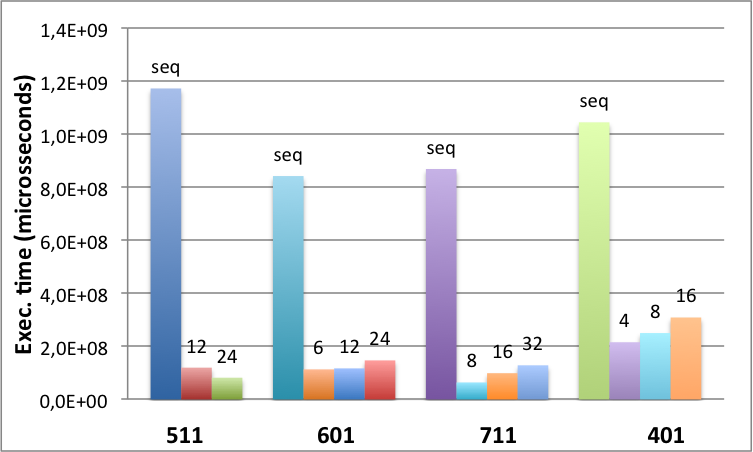
\includegraphics[scale=0.6]{../../common/graphs/exec_times_pointer.png}}
		\raisebox{-0.5\height}{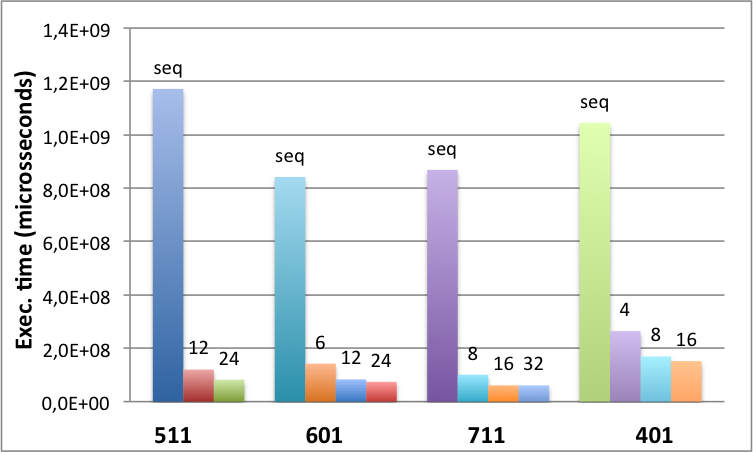
\includegraphics[scale=0.6]{../../common/graphs/exec_times_nonpointer.png}}
		\caption{Execution times of the \tth application for pointer static (left) and non-pointer dynamic (right) scheduler implementations for 512 variations.}
		\label{fig:ExecTimes}
	\end{center}
\end{figure}

Figure \ref{fig:ExecTimes} presents the execution time for all test systems. For each system, the bars represent, from left to right, the original application, parallel with number of threads equal to the number of cores in one CPU, number of threads equal to the total number of physical cores and number of threads equal to the total number of cores with multithreading, if available. For the pointer version, the best system is the compute-711 for 8 threads. The compute-511 system is the second best for 24 threads. However, it presents the worst efficiency as it has more physical cores than any other system. The best overall results occur when using the non-pointer version with all available hardware threads for the compute-711. Note that the compute-711 is the most recent high end system of all tested. The slower system is the compute-401, which is also the oldest and with fewer cores and smaller memory bandwidth. All the systems present the same behavior: for the pointer version, the execution time increases when using more than one CPU, due to the hazardous non unified memory accesses; for the non-pointer version, the execution time diminishes with the increase of threads, with hardware multithreading slightly increasing the performance due to better resource usage.

\section{Using the \nvidia CUDA/GPU accelerator}
\label{Parallelization:GPU}

Programming for GPUs still presents a series of important limitations imposed by the drivers due to the hardware characteristics. It uses C language for programming and it is not possible to use C++ classes. Also, libraries must be programmed specifically for the hardware accelerator, which prevents the use of any functions of LipMiniAnalysis and ROOT frameworks. This restricts the region of \ttDilepKinFit suitable to parallelize on GPU due to many dependencies on ROOT functions and classes.

The variation computation and kinematical reconstruction uses the \texttt{TLorentzVector} class from ROOT for holding the Bottom Quarks and leptons information. They have the particularity of always being executed, unlike the Higgs Boson reconstruction. However, it is possible to eliminate these dependencies, but causing an additional overhead. The other parts of \ttDilepKinFit are heavely dependent on ROOT and are not possible to port to GPU. Considering these factors, a parallel workflow was devised and is presented in figure \ref{fig:GPUPipeline}. The implementation details are presented in subsection \ref{GPUImplementation}. 

\begin{figure}[!htp]
	\begin{center}
		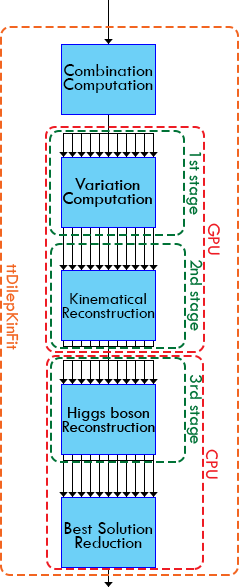
\includegraphics[scale=0.5]{../../common/img/gpu_pipeline.png}
		\caption{Schematic representation of the \ttDilepKinFit workflow on GPU.}
		\label{fig:GPUPipeline}
	\end{center}
\end{figure}

Similar to the shared memory parallelization, selecting all the combinations of Bottom Quark jets and leptons is a serial task. Then, a process of data marshalling is applied to transform all the information on the \texttt{TLorentzVector} classes into standard arrays. These arrays must be copied to the GPU memory so that the variation can be applied. The Mersenne Twister implementation available in the \nvidia cuRand library is used as the pseudo-random number generator (already discussed in section \ref{InitialOptimizations}). Then, the kinematical reconstruction is performed and the results are transferred back to the CPU memory. In the CPU, the data unmarshalling, i.e., transforming the results from the arrays into the ROOT classes to be used by the rest of the application, is performed and the Higgs Boson reconstruction is parallelized on the CPU.

There are several factors which will restrict the performance. The data marshalling and unmarshalling will add a sginificant overhead to \ttDilepKinFit, but it cannot be avoided. Even though the amount of data to transfer is small, with a similar size to the data structure used in the shared memory implementation, it occurs for every event and the kernel execution can only begin after all the data is copied. Assynchronous memory transfers can be used but they will not benefit the performance as it forces blocks of threads to run serialized to others, limited by the combinations that arrive to the GPU memory. It would increase the performance if all the threads would work on the data as it arrives, but that is not the case with this algorithm. The kernel itself is very complex with the variations and kinematical reconstruction. The computations are not homogeneous, with many operations performed in different data, which will result in a very high resource usage (namely registers and L1 cache). Register spilling might limit the performance as high register usage is an inherent characteristic to the kernel and cannot be optimized. Finally, the data structure used in the shared memory implementation is also present, as it is used to store all the combinations, so that they can be marshalled and transferred to the GPU memory, and is later used in the parallel Higgs Boson reconstruction. The best solution merge is also a required step.

During the GPU execution, the CPU is idle waiting for the results, and vice-versa. This inefficient usage of the computational resources is caused by the inexistence of a data structure holding all the event information. Figure \ref{fig:GPUExecFlows} presents the current and optimal execution flows between CPU and GPU. The optimal flow could be implemented if the event data was loaded to a data structure, rather than overwritting all information on memory. This would require a restructure of the application and LipMiniAnalysis, which is not possible in the timeframe of this dissertation work, but could render the usage of hardware accelerators a valid option for event processing.

\begin{figure}[!htp]
	\begin{center}
		\raisebox{-0.5\height}{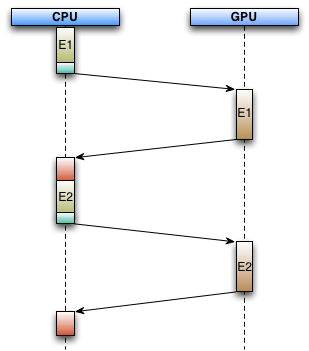
\includegraphics[scale=0.6]{../../common/img/gpu_flow.png}}
		\raisebox{-0.5\height}{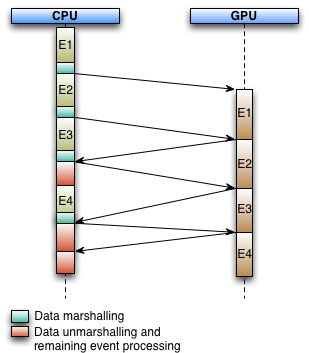
\includegraphics[scale=0.6]{../../common/img/gpu_optimal_flow.png}}
		\caption{Execution flows for the implemented workflow (left) and optimum workflow (right) of the \tth application.}
		\label{fig:GPUExecFlows}
	\end{center}
\end{figure}

\subsection{Implementation}
\label{GPUImplementation}

The data marshalling is performed on the data structure built when selecting the combinations, using the same process as with the shared memory parallelization implementation. On the variation computation and kinematical reconstruction, the most important data is the energy, mass and momentums of the Bottom Quark jets and leptons on the combination. The energy and momentums are double precision float point values of the \texttt{TLorentzVector} class, while the mass is computed based on those values. The mass function was copied from the ROOT source code to be implemented on GPU. The rest of the information is copied to various arrays, one per each particle. Other data, such as 4 \texttt{TLorentzVectorWFlags} class instances per event, from the LipMiniAnalysis library, and other control information (scalars) are also copied to specific arrays.

The variation computation uses the Mersenne Twister algorithm available in the \nvidia cuRand library \cite{NVIDIA:cuRand}, which produces uniformly distributed pseudo-random numbers. The transformation algorithm used in the ROOT \texttt{TRandom3} class, to map the values from a uniform to gaussian distribution, was ported from the ROOT source code to the GPU. The objective is to keep the changes in the \ttDilepKinFit algorithms to a minimum. One precomputed state was used per block of threads for the Mersenne Twister algorithm, which allows up to 256 threads to simultaneously generate pseudo-random numbers. The required numbers are generated at the beginning of the variation function, so that all the calls to the generator occur simultaneously, increasing the parallelism which benefits this kind of hardware accelerators.

Both the variation computation and kinematical reconstruction source code was modified to work on the input arrays, rather than resorting to ROOT classes. The results of the kinematical reconstruction are also stored in an array. However, since the kinematical reconstruction can return none, two or four instances of the \texttt{TLorentzVector} class, depending on the solution found, it is necessary an additional array to store the output size of each thread. Without this information, solutions can be assigned to the wrong combinations during the data unmarshalling. The varied parameters are also copied to the CPU memory and the data structure is updated.

The parallelization of the Higgs Boson reconstruction was implemented using OpenMP, with the dynamic scheduler as the workload is irregular since some variations of the combinations might not be reconstructable. The best solution merge is similar to the one presented in section \ref{SharedMemImplementation}.

\begin{figure}[!htp]
	\begin{center}
		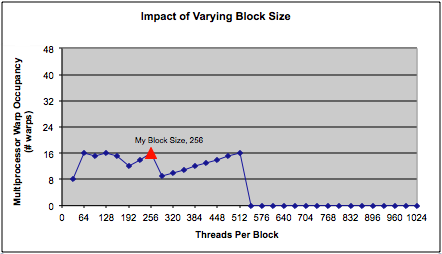
\includegraphics[scale=0.6]{../../common/graphs/block_size_gpu.png}
		\caption{Optimal number of threads for the GPU kernel, according to the \nvidia CUDA Occupancy Calculator.}
		\label{fig:GPUCalc}
	\end{center}
\end{figure}

The number of threads per block is limited to 256 due to the pseudo-random number generator restraints. The best block size for a kernel can be calculated using the \nvidia CUDA Occupancy Calculator \cite{NVIDIA:Calculator}, and depends on the number of registers that the kernel uses, the GPU architecture and cache size. The result of the calculation is presented in figure \ref{fig:GPUCalc}, which indicates that the best configuration uses 256 CUDA threads per block. The number of CUDA threads is equal to the number of variations times combinations, which varies between events, and, if possible, the threads may be organized in blocks of 256.

\subsection{Performance analysis}
\label{GPUPerformance}

The GPU implementation was tested in the compute-511 system with a \nvidia Tesla C2050\footnote{See appendix \ref{App:TestEnv} for more hardware details.}. The focus is on evaluating the limiting factors as it was not expected great performance due to the details already referred in \ref{Parallelization:GPU}.

\begin{figure}[!htp]
	\begin{center}
		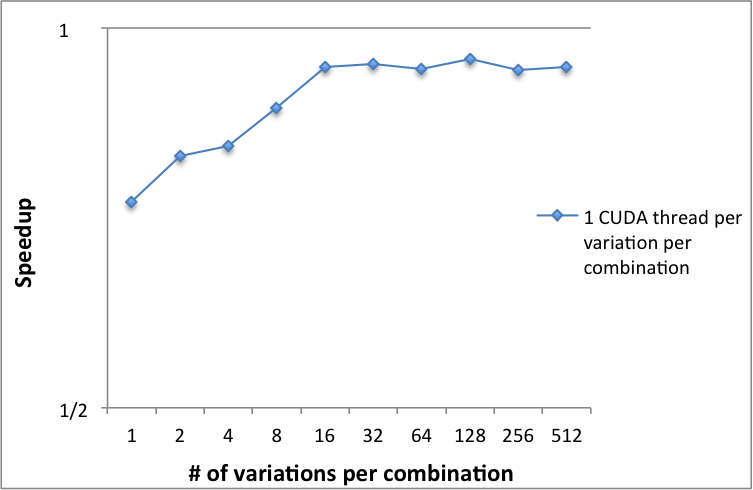
\includegraphics[scale=0.7]{../../common/graphs/speedup_gpu.png}
		\caption{Speedup of the \tth application for the GPU parallel implementation.}
		\label{fig:GPUSpeedup}
	\end{center}
\end{figure}

Figure \ref{fig:GPUSpeedup} illustrates the speedup for this implementation. For all different variations tested, the implementation is always slower than the original application. All the data (un)marshalling, transfer and unefficient usage of resources greatly restricts the potential performance gains.

\begin{figure}[!htp]
	\begin{center}
		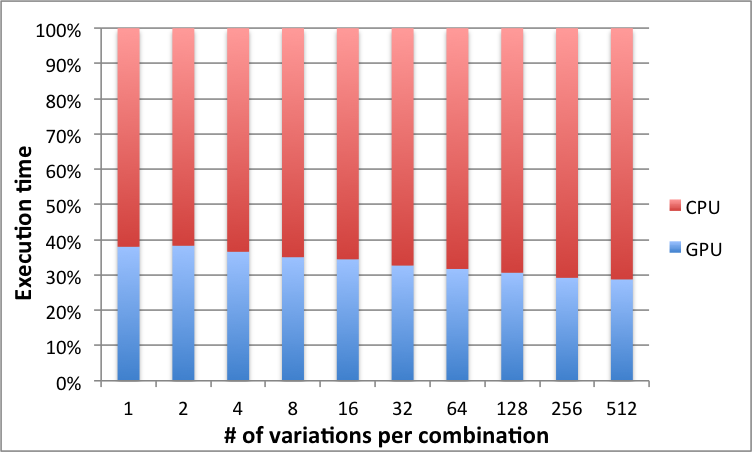
\includegraphics[scale=0.7]{../../common/graphs/percentage_time_gpu.png}
		\caption{Relative execution time of \tth application on CPU and GPU.}
		\label{fig:GPUPercentage}
	\end{center}
\end{figure}

Figure \ref{fig:GPUPercentage} shows the relative execution time of the application that is spent on the GPU and on the CPU. Since the CPU and GPU cannot work simultaneously, the graph also shows the percentage of time that each of the resources is idle. On average, the GPU is idle 70\% of the time, wasting important computational resources. Before optimizing memory transfers or the kernel itself, the low GPU usage is the main bottleck in which most efforts must be focused.

Even though the speedups do not motivate any efforts on optimizing this implementation, the low GPU usage is due to the global event data and a restructuration of the application, and LipMiniAnalysis library, would greatly improve the implementation. Introducing a data structure holding all the event information would allow the workflow presented in the right image of figure \ref{fig:GPUExecFlows} to be implemented and explore all the potential performance increase offered by the GPU.

\section{Using the \intel MIC Xeon Phi accelerator}
\label{Parallelization:MIC}

The \intel Xeon Phi has two operating modes. The native mode is supposed to run all the application on the device, requiring all code to be compiled with the \intel compiler and specific flags. In this mode, the device reserves one core to run the operating system, and it is required to copy all libraries, binaries and input files to the Xeon Phi memory prior to execution. In the offload mode the CPU operates the Xeon Phi as an accelerator, similar to GPUs. The objective is to do preliminary tests comparing both operating modes.

Since the native Xeon Phi execution model is similar to a multicore CPU, the workflow of the shared memory implementation is suitable for the problem. In theory, no changes to the shared memory implementation would be necessary to run on the device. Figure \ref{fig:MICWorkflows} illustrates the workflows for the native and offload device operative modes.

\begin{figure}[!htp]
	\begin{center}
		\raisebox{-0.5\height}{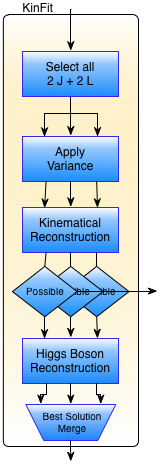
\includegraphics[scale=0.6]{../../common/img/parallel_kinfit.png}}
		\raisebox{-0.5\height}{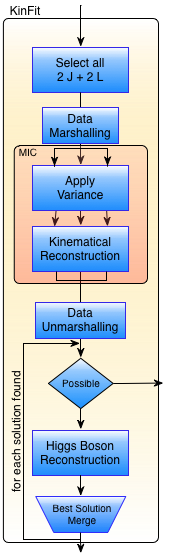
\includegraphics[scale=0.5]{../../common/img/mic_offload.png}}
		\caption{Workflows for the native (left) and offload implementation (right) on the \intel Xeon Phi.}
		\label{fig:MICWorkflows}
	\end{center}
\end{figure}

For the offload mode, the implementation will suffer from the same problems as the GPU implementation. For each event, it is required to copy the data structure holding all the combination information. Even though it is possible to use C++ classes on the accelerator, it is not possible to have a library simultaneously compiled for the CPU and Xeon Phi without modfying the source code. However, that is not possible to do in the ROOT and LipMiniAnalysis libraries within the timeframe of the dissertation work. This restricts the region of the application to parallelize on the Xeon Phi to only the variations computation and kinematical reconstruction. Also, by not using the ROOT classes, the same data (un)marshalling processes used in the GPU implementation are required. The Higgs Boson reconstruction is performed in parallel on CPU. This implementation was performed using the \intel compiler directives, avoiding the overhead added by using MPI, which is also based on these directives.

The resource usage efficiency will be similar to the GPU implementation, where the CPU is idle when the Xeon Phi is computing, and vice-versa. The purpose is to evaluate the usability of the accelerator, as \intel claims that porting (unefficient) code to the device is straight forward.

\subsection{Implementation}
\label{MICImplementation}

The implementation for the Xeon Phi native operating mode requires the compilation of the ROOT library, since both LipMiniAnalysis and the application depends on it. ROOT offers specific compilation for \intel Xeon Phi devices, developed by CERN OpenLab. However, it does not work on the compute-711 test system. Much of the development time for this implementation was spent trying to solve the bug on the many ROOT makefiles. However, since the device is much simpler than the CPU and only runs at 1 GHz, it would not offer a significant performance gain relatively to the CPU shared memory implementation, even with the larger throughput of the device. Therefore, this implementation was left on hold to be continued later on.

The parallel GPU implementation was adapted to run on the Xeon Phi in offload mode, with requiring many modifications modifications. Where each CUDA thread would process one variation per combination, on the Xeon Phi these tasks are grouped to match the device threads. The data (un)marshalling is similar to the GPU implementation and the data transfers are implemented using compiler pragma directives. These directives offer a simple way to implement the data transfers but only work with standard C structures, such as arrays.

Even though the Xeon Phi was already tested with static benchmarks and relatively simple algorithms, the drivers offered huge limitations for the implementation of such complex algorithms. During the preliminary implementation, the drivers returned many different errors when offloading the functions that did not even got a description. \intel support advised to look into headers of the respective sections of the drivers to help identify the errors source. The implementation was stalled by a timeout error from the driver that was left unsolved, even though the device was properly installed and was fully working according to the \intel control tools.

Both native and offload implementations were left on hold since it was for the LIP research group best interest to focus on the shared memory and application scheduler implementations.

\section{Using an application scheduler}
\label{Parallelization:Scheduler}

The idea for an application scheduler derived from the high performance and efficiency delivered by the shared memory pointer implementation running on a single CPU. Huge amounts of eventy data files, which usually have 1 GB size, need to be processed everytime a new batch arrives from the Tier-2 computational centers. This scheduler is an application that manages the execution of those files among a given amount of the same, or different, applications. As an example, instead of using one application to execute with 16 threads on the compute-711 system (consider the shared memory implementation on section \ref{Parallelization:SharedMem}), two applications with 8 threads of the pointer version could run simultaneously, providing better resource usage and process the same amount of data in less time.

\begin{figure}[!htp]
	\begin{center}
		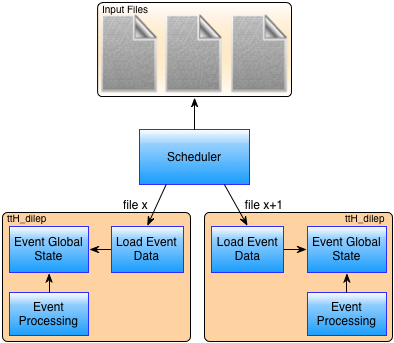
\includegraphics[scale=0.7]{../../common/img/scheduler_workflow.png}
		\caption{Schematic representation of the application scheduler.}
		\label{fig:SchedulerWorkflow}
	\end{center}
\end{figure}

Figure \ref{fig:SchedulerWorkflow} presents the schematic representation for the proposed scheduler workflow designed for a shared memory environment. Although it will be tested with the parallel shared memory implementation (pointer version, due to its efficiency) of the \tth application, it is designed to virtually work with any kind of application and input data files. The scheduler is tuned and configured by the following set of parameters:

\begin{description}
	\item[Application:] the name of the binary file of the application, or applications, to execute.
	\item[Input parameters:] the input parameters of the applications to execute, without the input data file specified. Multiple parameters are required if different applications are used.
	\item[Input data files:] range of the input data files to process. They are usually numbered (for example sample\_001 to sample\_500). Multiple files can be specified if different applications are used.
	\item[Number of applications:] the maximum number of applications running simultaneously on the system.
	\item[Threads:] the number of threads to run per application. A standard way to set the threads must be implemented by the application. If it uses OpenMP, it is possible to do so by setting environment variables.
\end{description}

The amount of applications to run simultaneously, and the number of threads per each application, will directly affect the performance of the scheduler. If not properly configured, it can lead to resource starvation, in the case that the total number of threads/applications is not enough to use all available resources, or overwhelm the system resources, where a high number of threads is used. At the moment, the best configuration can only be obtained by benchmarking the application and different configurations for the scheduler on the specific system to test.

The purpose of the scheduler is to provide a simple way of increasing the usage of the available computational resources to be without requiring the know-how of the underlying concepts of parallel programming. For the scheduler to be adopted by the physicists it needs to be easy to interact with and offer a considerable performance increase. A proper scheduling technic would require the use of micro-benchmarks, with similar characteristics of the applications, to assess the best configuration parameters. It would be necessary to study the different applications characteristics and chose adequate micro-benchmarks for each situation, allowing the scheduler to provide the best configuration for the system. Since this is only one of many proposed parallelization strategies, there was only time to develop a prototype, which needs to be manual tuning and configuration for each system.

Each input data file has a set of different events, meaning that the execution of the same application with different files is irregular. This irregularity benefits the usage of a dynamic load balancing strategy rather than a static, if the overhead of the first is low enough to not restrict the performance. An application execution is never less than a few seconds, providing a coarse task granularity. This means that the overhead induced by using a dynamic load balance strategy is not relevant compared to the time that takes to process a parallel task.

\subsection{Implementation}
\label{SchedulerImplementation}

Even though the application scheduler was designed considering many of features presented in section \ref{Parallelization:Scheduler}, it was only possible to develop, within the dissertation timeframe, a prototype to serve as a proof of concept. The scheduler is fully operational but with some limitations, later explained, needing more features to be implemented and refined before being ready for physicists to use.

The current prototype reads the configurable parameters from a text file (an example file is presented in \ref{fig:SchedulerFile}). This file is read at the beginning of the scheduler execution and will affect its behavior and performance. The prototype is only prepared to read and parse the configuration file for running one application with the same set of parameters, but with different input data files.

\begin{figure}[!htp]
	\begin{center}
		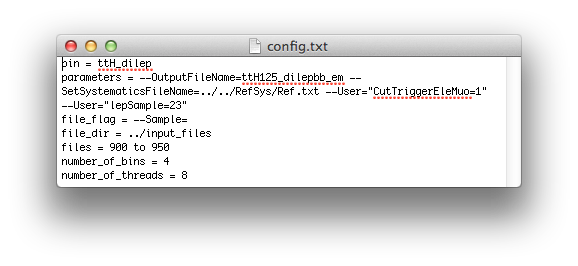
\includegraphics[scale=0.8]{../../common/img/scheduler_config.png}
		\caption{Example scheduler configuration file.}
		\label{fig:SchedulerFile}
	\end{center}
\end{figure}

The file structure is simple and intuitive but it was only designed for applications similar to \tth. The order of the parameters is irrelevant as long as they are properly identified. \textit{bin} and \textit{parameters} refer to the name of the binary file of the application and its parameters, without the flag specifying the file to process. The files are indicated in the \textit{files} field, where they can be enumerated or use the \textit{to} connector that indicates all the files between the files \textit{900} and \textit{950}. The \textit{file\_dir} and \textit{file\_flag} field indicate the directory in which the files are stored and the flag used by the application to specify the file to process, respectively. \textit{number\_of\_bins} and \textit{number\_of\_threads} indicate the amount of applications to run simultaneously and the number of threads per application. In the specific case of this application it is possible to define by an environment variable the number of variations per combination.

A data structure is created holding the information for each application execution (considered as an element of the structure), which size is equal to the number of input data files to process. The string with the application parameters is concatenated with the input data file flag and name and stored in the structure. Also, each element of the structure has the number of threads associated. This allows the scheduler to be abstract enough to work with different applications with irregular parameters and different number of threads. The number of threads of the application is set through environment variables, when it is prepared to be executed, as the parallel \tth application is implemented using OpenMP and it allows set the threads in this way.

OpenMP was used to parallelized the applications execution. The number of threads is equal to the number of applications to run simultaneously, as each thread is responsible for the its application setup and execution. The threads operate in a work stealing pattern, getting hold of an element of the scheduler data structure and processing it, until the data structure is swept. The OpenMP dynamic scheduler is used as it is designed to efficiently handle this kind of irregular load and its overhead is not significant compared to each application execution time.

The implementation of micro-benchmarks to infer the best configuration of the scheduler would depend on the computational characteristics of the applications to manage. The tests performed in subsection \ref{SchedulerPerformance} are based on the parallel \tth performance analyzed on section \ref{SharedMemPerformance}, but this might not valid for other test systems and applications. The benchmarks could be synthetic algorithms designed to evaluate the system performance, which need to be adequate to this type of applications, or the application itself running with one of the input data files, but it would be encessary to guarantee that its execution time is low. The latter alternative would induce an higher overhead but could provide a more accurate evaluation of the test system.

Little changes to the configuration file would be necessary to consider multiple different applications. Its structure is modular, so, to insert a different application, the fields in figure \ref{fig:SchedulerFile} would be replicated. This would also require little changes to the current parser on the scheduler and the data structure is already prepared to deal with any kind of application.

\subsection{Performance Analysis}
\label{SchedulerPerformance}

The performance analysis of the scheduler prototype is presented in this section. All tests are performed on the compute-711 system using the \tth application, with a set of 10 input data files and various numbers of variations per combination. The scheduler runs the most efficient parallel implementation of \tth, the pointer version, avoiding the use of NUMA accesses as each application will have enough cores in one CPU to process its threads. Different combinations of number of simultaneous applications and threads per application are compared agains the original \tth and non-pointer parallel implementation using the same total number of threads (for example, 4 applications with 4 threads \textit{vs} single application wiht 16 threads), as it is the fastest using both CPUs on the system.

\begin{figure}[!htp]
	\begin{center}
		\raisebox{-0.5\height}{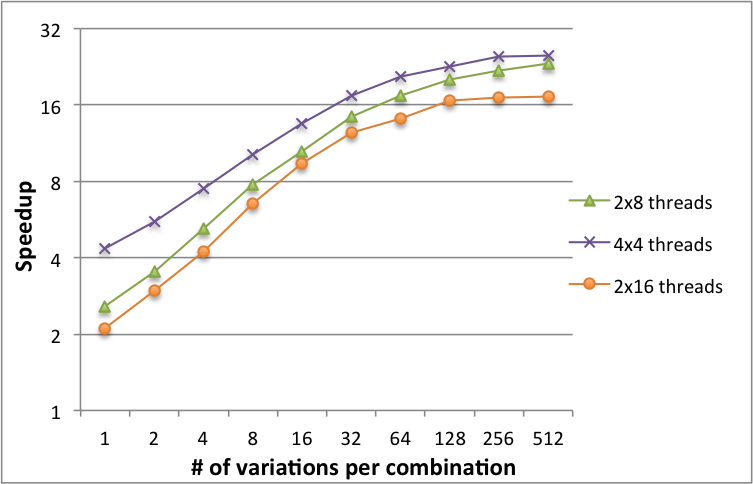
\includegraphics[scale=0.6]{../../common/graphs/speedup_scheduler.png}}
		\raisebox{-0.5\height}{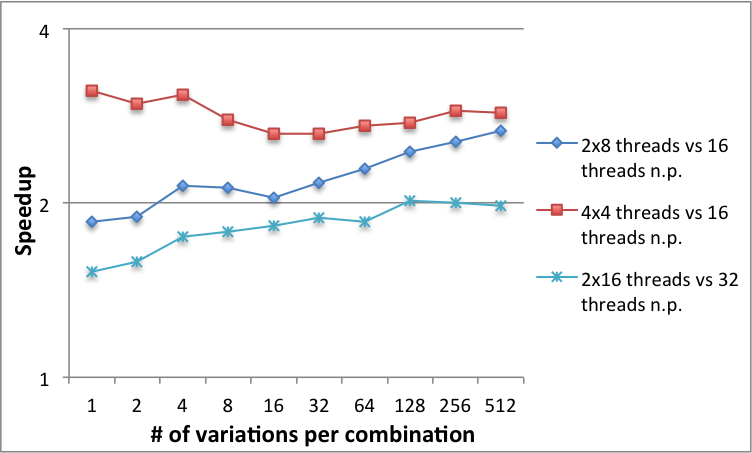
\includegraphics[scale=0.64]{../../common/graphs/speedup_scheduler_vs_np.png}}
		\caption{Speedup of the scheduler with different setups (simultaneous applications \textit{x} number of threads per application) versus the original application and the non-pointer (n.p.) parallel implementation.}
		\label{fig:SchedulerSpeedups}
	\end{center}
\end{figure}

Figure \ref{fig:SchedulerSpeedups} presents the speedup of the scheduler for three setups compared to the original sequential application (left graph). The scheduler performance using 4 applications with 4 threads each (\textit{4x4}) and 2 applications with 8 threads (\textit{2x8}) is very similar, with a slight advantage for the first setup. It achieves a maximum speedup of 25 for 512 variations per combination, while the best performance achieved by the non-pointer parallel implementation, presented in section \ref{SharedMemPerformance}, has a speedup of 14.6. Note that the speedup is higher than the number of cores because of the PRNG optimizations are not implemented in the original application. The scheduler transposes the efficiency of the parallel pointer implementation on a single CPU to a dual-socket system. The advantage of the \textit{4x4} setup is due to the higher number of applications for the scheduler to manage, allowing for a better load distribution. The worst performance occurs for the \textit{2x16} setup, with all the hardware threads are used, plus 2 other threads are require by the scheduler to manage the applications execution. The use of hardware multithread does not benefit the parallel pointer implementation due to the use of pointers to shared data.

The graph on the right of figure \ref{fig:SchedulerSpeedups} presents the speedup of the 3 setups of the scheduler compared to the non-pointer parallel implementation for the same total number of threads. The best performance increase occurs for the \textit{4x4} setup, with a relatively constant speedup of 3 for all different variations. For the \textit{2x8} setup, the speedup increases with the number of variations, with similar behavior for the \textit{2x16} setup. Overall, the scheduler with the parallel pointer implementation offers better performance and, consequently, more efficient resource usage than the best implementation for shared memory.

\begin{figure}[!htp]
	\begin{center}
		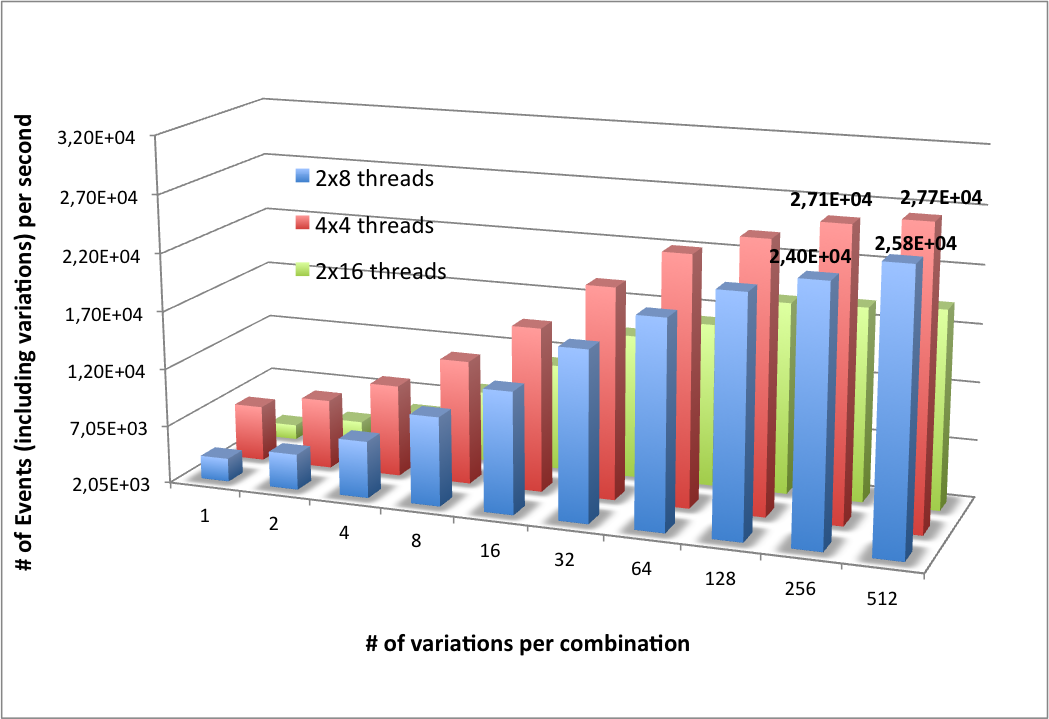
\includegraphics[scale=0.7]{../../common/graphs/throughput_scheduler.png}
		\caption{Event processing throughput for various number of variations and different scheduler setups.}
		\label{fig:SchedulerThroughput}
	\end{center}
\end{figure}

The highest event throughput, presented in figure \ref{fig:SchedulerThroughput}, occurs for the \textit{4x4} setup, as expected from the observed speedups, with 27700 events processed per second for 512 variations. The \textit{2x8} setup has a peak throughput of 25800 events per second, close to the \textit{4x4} setup. The highest throughput for a single parallel implementation was 14300 events per second, presented in figure \ref{fig:EventThroughput}. The scheduler provides almost a two-fold increase in event processing, presenting itself as the most viable option for processing in a dual-socket system.
